\documentclass[border=10pt]{standalone}

\usepackage{tikz}
\usepackage{tikzsymbols}
\usetikzlibrary{calc,patterns,shapes.geometric}

\def\centerarc[#1](#2)(#3:#4:#5){\draw[#1] ($(#2)+({#5*cos(#3)},{#5*sin(#3)})$) arc (#3:#4:#5);}

\begin{document}
	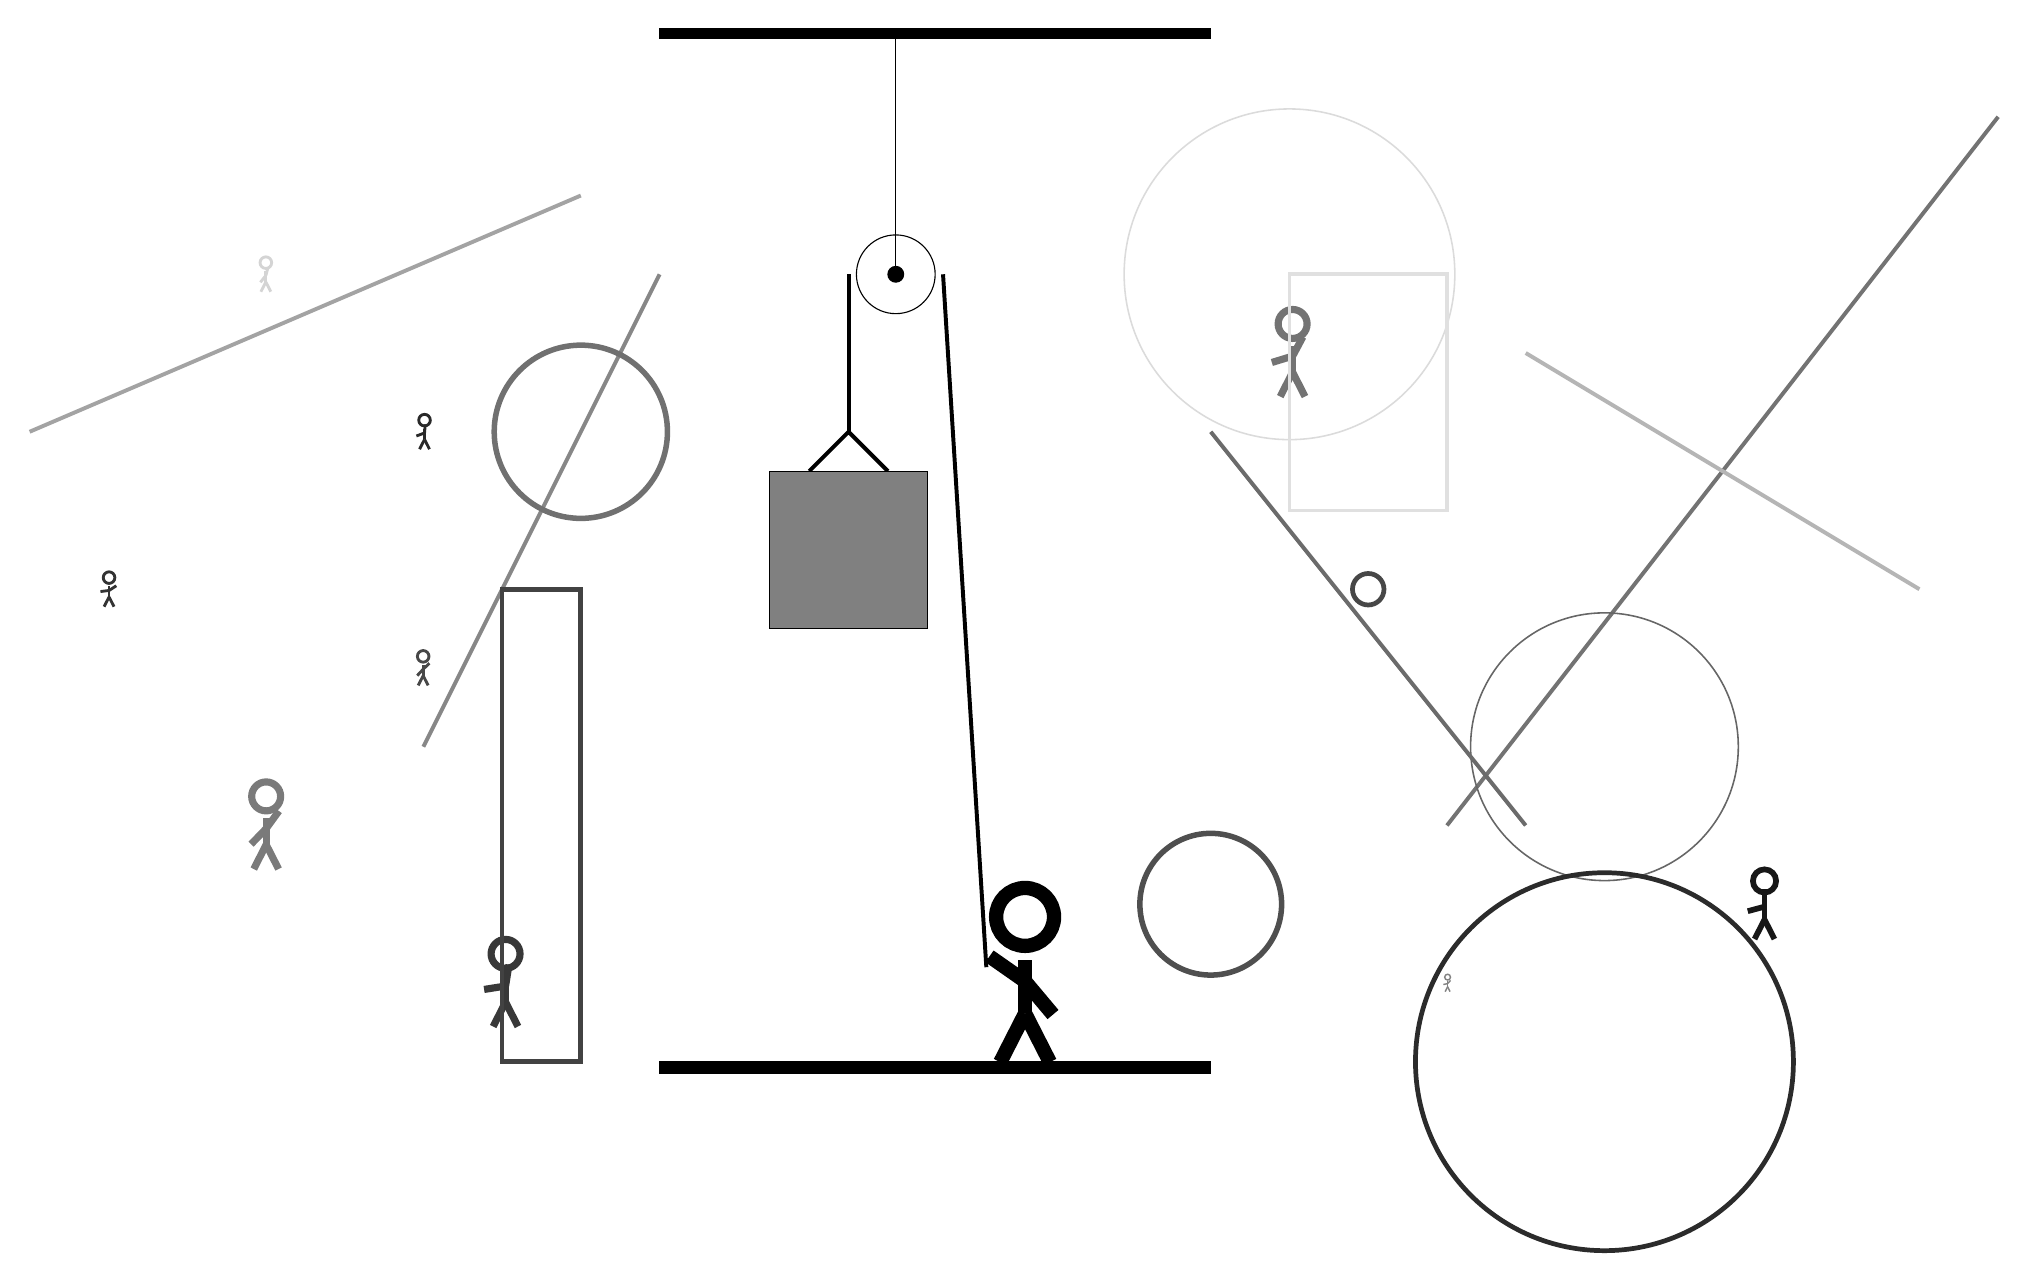
\begin{tikzpicture}
		%%%%% START %%%%%
		
		\draw[fill=black] (-2, 10) rectangle (5, 10.125);
		
		\draw [line width=0.6mm, color=black!72](7, 3) circle (0.2);
		
		\node[line width=0.2mm, color=black!84] at (-5, 5) {\Strichmaxerl[2][20][85]};
		\node[line width=0.7mm, color=black!17] at (-7, 7) {\Strichmaxerl[2][51][75]};
		\draw[line width=0.5mm, color=black!38](6, 7) -- (6, 4);
		\draw[line width=0.5mm, color=black!55](8, 0) -- (15, 9);
		\node[line width=0.6mm, color=black!80] at (-9, 3) {\Strichmaxerl[2][7][33]};
		\node[line width=0.3mm, color=black!78] at (-4, -2) {\Strichmaxerl[5][9][81]};
		
		\node[line width=0.3mm, color=black!91] at (12, -1) {\Strichmaxerl[4][15][90]};
		\draw[line width=0.5mm, color=black!47](-5, 1) -- (-2, 7);
		\draw [line width=0.2mm, color=black!14](6, 7) circle (2.1);
		\draw [line width=0.2mm, color=black!60](10, 1) circle (1.7);
		\node[line width=0.4mm, color=black!55] at (6, 6) {\Strichmaxerl[5][17][62]};
		\draw[line width=0.5mm, color=black!36](-3, 8) -- (-10, 5);
		
		\draw [line width=0.7mm, color=black!56](-3, 5) circle (1.1);
		\draw[line width=0.5mm, color=black!12] (6, 4) rectangle (8, 7);
		\draw[line width=0.5mm, color=black!29](9, 6) -- (14, 3);
		\draw [line width=0.7mm, color=black!69](5, -1) circle (0.9);
		\node[line width=0.6mm, color=black!49] at (8, -2) {\Strichmaxerl[1][13][47]};
		\node[line width=0.7mm, color=black!72] at (-5, 2) {\Strichmaxerl[2][47][44]};
		\node[line width=0.7mm, color=black!52] at (-7, 0) {\Strichmaxerl[5][46][54]};
		\draw [line width=0.6mm, color=black!83](10, -3) circle (2.4);
		\draw[line width=0.5mm, color=black!58](5, 5) -- (9, 0);
		\draw[line width=0.6mm, color=black!74] (-4, -3) rectangle (-3, 3);
		
		\draw (1, 7) circle (0.5);
		\draw[fill=black] (1, 7) circle (0.1);
		\draw (1, 10) -- (1, 7);
		
		\draw[line width=0.5mm] (-0.1, 4.5) -- (0.4, 5.0) -- (0.9, 4.5);
		\draw[fill=black!50] (-0.6, 4.5) rectangle (1.4, 2.5);
		
		\draw[line width=0.5mm] (0.4, 7) -- (0.4, 5.0);
		\centerarc[line width=0.5mm](1, 7)(0:180:0.6);
		\draw[line width=0.5mm](1.6, 7) -- (2.15, -1.8);
		
		\node at (2.6, -1.9) {\Strichmaxerl[10][-35][-50]};
		
		\draw[fill=black] (-2, -3) rectangle (5, -3.15);
		
		%%%%% END %%%%%
	\end{tikzpicture}
\end{document}